% --- Documentclass specifications ---
\documentclass[italian]{tktltiki2}
\linespread{1.3}

% --- General packages ---
\usepackage[utf8]{inputenc}
\usepackage[T1]{fontenc}
\usepackage{lmodern}
\usepackage{epigraph}
\usepackage{microtype}
\usepackage{amsfonts,amsmath,amssymb,amsthm,booktabs,color,enumitem,graphicx}
\usepackage[pdftex,hidelinks]{hyperref}
% setting C language style listing
\usepackage{listings}
\lstset{
  language=C,
  basicstyle=\fontsize{8}{11}\selectfont\ttfamily
}
% Automatically set the PDF metadata fields
\makeatletter
\AtBeginDocument{\hypersetup{pdftitle = {\@title}, pdfauthor = {\@author}}}
\makeatother

% --- Language-related settings ---
\usepackage[fixlanguage]{babelbib}
% add bibliography to the table of contents
\usepackage[nottoc]{tocbibind}


% --- tktltiki2 options ---
%
% The following commands define the information used to generate title and
% abstract pages. The following entries should be always specified:
\title{%
  \huge Project Heimdall \\
  \large Proposta di implementazione per un web switch \\ 
    concorrente two-way di livello 7 (OSI) con \\
    politiche di bilanciamento del carico stateless e stateful
  }
\author{\emph{Alessio Moretti} - 0187698 \\\emph{Andrea Cerra} - 0167043\\\emph{Claudio Pastorini} - 0186256}
\date{\today}
\level{Corso di Ingegneria di Internet e del Web - A.A. 2014/2015}
\university{\textbf{Università degli studi di Roma Tor Vergata}}
\department{\textbf{Facoltà di Ingegneria Informatica}}
\city{Roma}

\begin{document}

% --- Front matter ---
\maketitle        % title page

\tableofcontents  % table of contents
\pagenumbering{gobble}

% --- Main matter ---
\mainmatter       % clear page, start arabic page numbering

\section{Example section}
% Example of a quote
\begin{quote}
\flushright
	\emph{Yggdrasil, l'albero del mondo, che congiunge i nove regni del cosmo con Asgard, la dimora degli dei.} \\ Heimdall, custode del Bifröst
\end{quote}

% Write some science here
Sample text and a reference\cite{lamport94}. Lorem ipsum dolor sit amet, consectetur adipiscing elit. Donec at lorem varius, sodales diam semper, congue dui. Integer porttitor felis eu tempor tempor. Proin molestie maximus augue in facilisis. Phasellus eros dui, blandit eu nibh ut, pharetra porta enim. Cum sociis natoque penatibus et magnis dis parturient montes, nascetur ridiculus mus. Aliquam ullamcorper risus pretium est elementum, eget egestas lorem fermentum. Etiam auctor nisi purus, vitae scelerisque augue vehicula sed. Ut eu laoreet ex. Mauris eu mi a tortor gravida cursus eget sit amet ligula.

\begin{figure}
\centering

\includegraphics[width=\textwidth]{images/thor}
\caption{Thor di Asgard, \emph{figlio di Odino}}
\end{figure}

\newpage
\section{Introduzione}
\subsection{Perché Heimdall?}
Heimdall è il personaggio dell'universo Marvel, ispirato all'omonimo dio della mitologia norrena, egli è il guardiano del regno di Asgard e del Bifröst. Quest'ultimo è il ponte che unisce la Terra alla dimora degli dei ed Heimdall, come suo custode, ha il compito di aprirlo ed indirizzarlo verso gli altri mondi, permettendo solamente a chi è degno di attraversare le distese dello spazio. \\
Ci piace pensare che questo sia un po' il ruolo del software nato dal nostro progetto: che sia in grado di scegliere come meglio indirizzare le connessioni in arrivo, ponendosi come ``guardiano'' di un cluster di server che fa ad esso capo. Quindi un \textbf{web switch} che sia funzionale sia per ricevere o trasmettere pacchetti di un regolare traffico HTTP, che per bilanciare il carico dello stesso traffico in arrivo sulle varie macchine.

\subsection{Web switch di livello 7}
Nella terminologia delle reti informatiche uno \textbf{switch} è un commutatore a livello datalink, ovvero un dispositivo che si occupa di instradare opportunamente, attraverso le reti LAN, selezionando i frame ricevuti e reindirizzandoli verso la macchina appropriata a seconda di una propria tabella di inoltro. Un \textbf{web switch}, a livello applicativo, è capace di reindirizzare i dati in funzione dei pacchetti che riceve, analizzandone il contenuto e decidendo opportunamente la destinazione, occupandosi allo stesso tempo di reinoltrare anche l'eventuale risposta della macchina selezionata verso il client che l'ha generata. \\
Le applicazioni sono molteplici per l'implementazione a livello applicativo: può essere considerato un \textbf{proxy}, oppure, selezionando opportunamente la macchina con più velocità di risposta o con minore pressione, può agire come \textbf{bilanciatore di carico}. Infatti ognuno dei client che fa richiesta, ad esempio, per uno specifico sito web, invia un pacchetto ad un indirizzo IP pubblico che corrisponde a quello del nostro switch applicativo. Questi, dopo aver correttamente letto il pacchetto, si occupa di consultare una tabella di inoltro generata con una determinata \textbf{politica di scheduling} e quindi gestire l'inoltro della richiesta ed il reinoltro della risposta del webserver. Tutto questo in maniera totalmente trasparente al client, qualsiasi sia la macchina che ha effettivamente risposto, che sia un web server oppure un cluster di macchine associate ad un ulteriore switch.

\begin{figure}
\centering
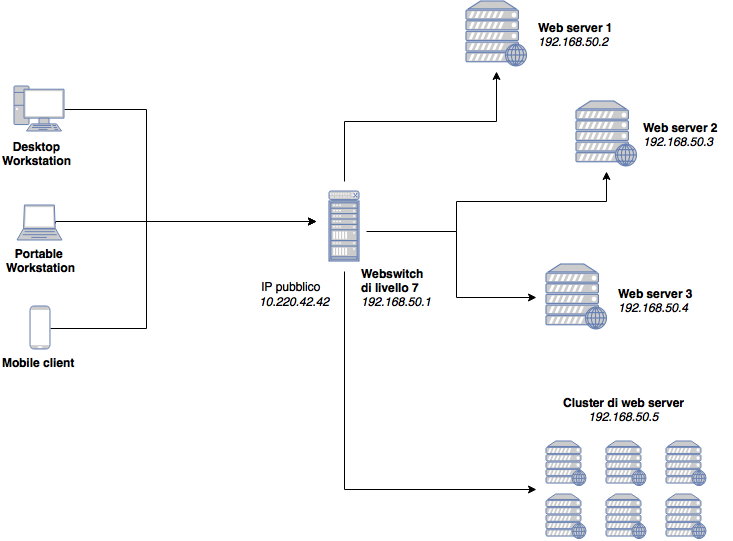
\includegraphics[width=\textwidth]{images/switch7}
\caption{Esempio di uno \emph{switch di livello 7 (OSI)}}
\end{figure}

\subsection{Web switch di livello 7}

\newpage
\section{Architettura}

\subsection{Server in ascolto}
\subsubsection{File di configurazione}
\label{sec:config}
\subsubsection{Logging}
\subsubsection{Gestione degli errori}

\subsection{Pool manager}

\subsection{Scheduler}

\subsection{Worker}
Il worker è il componente principale di Heimdall e non a caso gli è stato assegnato questo nome poiché è lui che ``lavora'' andando a servire le richieste dei client tramite lo smistamento ai vari server presenti nel cluster e il successivo inoltro delle risposte.
\\
Nell'attuale implementazione il worker è un processo composto da quattro thread: il \hyperref[sec:reader]{\emph{thread di lettura}}, il \hyperref[sec:writer]{\emph{thread di scrittura}}, il \hyperref[sec:request]{\emph{thread di richiesta}} e il \hyperref[sec:watchdog]{\emph{thread di watchdog}}.
\\
Heimdall è configurato in modo tale da effettuare il prefork di un numero configurabile di processi, questa scelta è stata fatta per evitare di aggiungere ritardo causato dal tempo di creazione di quest'ultimi.

\subsubsection{Gestione delle richieste}
L'applicazione soddisfa le specifiche HTTP 1.1 gestendo connessioni in modo persistente tramite pipeline. Questo vuol dire che da una stessa connessione TCP è possibile ricevere più di una richiesta HTTP (connessione persistente) senza dover necessariamente aver risposto alla richiesta precedente (pipeling). Per ottenere una connessione persistente abbiamo mantenuto aperta la connessione TCP anche dopo aver inviato la risposta e invece per ottere il pipeling abbiamo creato una coda delle richieste. 
Come detto pocanzi il worker è un processo che viene creato tramite prefork. Questo rimane in pause finché non gliene viene consegnata una connessione (una socket) tramite il message controller. Non appena ricevuta potrà iniziare a lavorare creando i vari thread necessari per 
\subsubsection*{Coda delle richieste}
Per poter supportare la tecnica del pipeling è stato necessario creare una coda delle richieste che contenesse tutte le richieste effettuate da un client tramite la stessa connessione HTTP. È stata implementata una coda poiché è necessario rispettare l'ordine delle richieste. 
La coda è molto semplice, è stata implementata:

La coda espone le seguenti operazioni:

All'interno della coda non sono presenti direttamente le richieste ma è stata creata un'ulteriore struttura, i request node. Questi nodi incapsulano al loro interno la richiesta, la risposta e (oltre a varie variabili di supporto per il multithreading) un'ulteriore struttura, il chuck. 
\subsubsection*{Chunk di dati}
\label{sec:chunk}
Un chunk è un ``pezzo'' che contiene parte della risposta. Parte, non la risposta completa dato che potrebbe essere anche una risosta corposa e quindi poter richiedere anche molto spazio. All'interno della struttura troviamo:

È stata fatta questa scelta per poter alleggerire al massimo il carico sul Web Switch che in questo modo non si dovrà appesantire con risorse ma che farà da passa carta tra server e client. Tramite questa soluzione siamo stati anche in grado di poter inviare la risposta in un tempo minore non dovendo aspettare necessariamente che il Web Switch abbia ricevuto completamente la risposta, in questo modo abbiamo ottenuto una risposta in tempi minori con il minor uso di memoria. Questo ci è stato possibile grazie alla natura dei socket che permettono la lettura e la scrittura contemporaneamente, come se lo stream di lettura fosse indipendente dallo stream di entrata.

disegnino socket con tubicini che non venivano usati contemporaneamente se non fosse stato usato il chunk -  utilizzo socket con chunck
\subsubsection{Gestione delle connessioni}
Il sistema è stato concepito per essere il più modulare possibile con valori di ritorno il più possibile uniformi. La gestione delle connessioni ne è un esempio lampante. Abbiamo realizzato un wrapping delle API Socket di Berkley in modo tale da gestire tutti gli errori allo stesso modo, tramite l'utilizzo dei Throwable. Oltre a questo abbiamo, fin dove possible, cercato di rendere più snella l'implementazione delle chiamate con  in modo tale da poterci preoccupare solo della logica dell'applicazione e non dalla sua effettiva implementazione. 
\subsubsection*{Connessione}
\subsubsection*{Richieste HTTP}
\subsubsection*{Risposte HTTP}
\subsubsection{Thread di lettura}
\label{sec:reader}
Il thread di lettura viene chiamato non appena il worker riceve una connessione da gestire. Questo thread ha il compito di leggere dal socket (tramite read bloccante) e di creare nodi da accodare alla coda delle richieste. Non appena ha accodato una nuova richiesta creerà il thread di richiesta, che chiamando un server sottostante, che si occuperà di gestire la richiesta. L'attuale implementazione fa un uso di un contatore per poter limitare il numero di richieste massime accettabili da una stessa connessione contemporaneamente. Quello che abbiamo notato dai nostri esperimenti è che Apache gestisce al massimo 100 richieste sulla stessa connessione, cosa che noi non limitiamo ma che rendiamo modificabile tramite l'apposita configurazione nel file config.
Il thread di lettura inoltre, ogni qual volta riceve una nuova connessione aggiorna un timer adibito alla verifica dello stato di vita della connessione ``si veda il paragrafo~\ref{sec:watchdog}.''
\subsubsection{Thread di scrittura}
\label{sec:writer}
Il thread di scrittura è adibito alla scrittura della risposta ottenuta tramite il thread di richiesta~\ref{sec:request}. Questi due thread cooperano per mezzo di una condition andando a scrivere e a leggere nella stessa area di memoria, il chunk~\ref{sec:chunk}. Dovendo rispondere in ordine il thread starà in loop sulla richiesta del fronte della coda e dopo aver inviato l'header di risposta (che non è gestito tramite chuck) 
\subsubsection{Thread di richiesta}
\label{sec:request}
Il thread di richiesta è adibito infine all'invio della richiesta ad un server nel cluster e alla successiva 
\subsubsection{Thread di watchdog}
\label{sec:watchdog}

\newpage
\section{Ulteriori proposte}

\newpage
\section{Politiche di scheduling}
La schedulazione permette la selezione della macchina predisposta a rispondere alla richiesta HTTP appena arrivata da parte del client, si basa su una tecnica nota come \textbf{bilanciamento del carico}, ovvero la distribuzione del carico, solitamente di elaborazione o di erogazione di uno specifico servizio, tra più server. Questo permette di poter \textbf{scalare} sulla potenza di calcolo del cluster dietro al web switch, lasciando che siano diverse macchine a rispondere a seconda di quella che è più veloce, più performante, oppure monitorando costantemente lo stato dei server e scegliendo quello meno sottoposto ad una pressione del carico di lavoro. \\ \\ 
Nella nostra implementazione \textbf{thread scheduler} si occupa di fornire,  ogni volta che viene invocato, una macchina selezionata secondo una delle due politiche che andremo ora a spiegare nel dettaglio più avanti.


\begin{figure}[b]
\centering
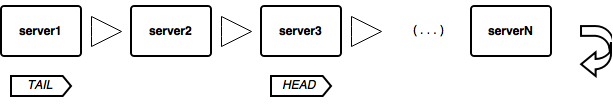
\includegraphics[width=\textwidth]{images/rrobin_stateless}
\caption{Schema di funzionamento del buffer circolare \label{fig: rrobin_sl}}
\end{figure}

\subsection{State-less: implementazione con Round-Robin}
L'algoritmo di scheduling Round-Robin (da adesso RR, \emph{n.d.r.}) è un algoritmo che agisce con prelazione distribuendo in maniera equa il lavoro, secondo una metrica stabilita in partenza. \\
L'algoritmo funziona utilizzando un buffer circolare come possiamo vedere in \hyperref[fig: rrobin_sl]{\emph{figura}}: questo permette di iterare la selezione su una lista di elementi precedentemente caricata. E' necessario quindi specificare due passi per il corretto funzionamento, dopo aver dato un rapido sguardo alla struttura che lo rappresenta nella nostra implementazione.\\\\
\begin{lstlisting}
typedef struct circular_buffer {
    Server      *buffer;
    int         buffer_position;
    int         buffer_len;
    
    Server      *head;
    Server      *tail;

    pthread_mutex_t mutex;

    ThrowablePtr (*allocate_buffer)(CircularPtr *circular, Server **servers, int len);
    ThrowablePtr (*acquire)(struct circular_buffer *circular);
    ThrowablePtr (*release)(struct circular_buffer *circular);
    void         (*progress)(struct circular_buffer *circular);
    void         (*destroy_buffer)(struct circular_buffer *circular);
} Circular, *CircularPtr;
\end{lstlisting}


\textbf{Inizializzazione del buffer:} in questa fase la struttura dati che rappresenta il buffer circolare, che mantiene due puntatori di \emph{testa} e \emph{coda}, viene inizializzata associandovi un array di puntatori di strutture di tipo \emph{Server} e viene eseguita la seguente funzione:
\begin{lstlisting}
    /* inside allocate_buffer ... */
    // allocating the buffer
    circular->buffer = *servers;
    circular->buffer_len = len;
    // setting params
    circular->head = circular->buffer;
    circular->tail = circular->buffer + (len - 1);
\end{lstlisting}
In un'ottica di \emph{produttore vs consumatore}
\subsection{State-aware: implementazione con monitor di carico}
\subsubsection{Modulo Apache Status}
Il modulo Apache Status (modstatus) è un modulo che fornisce informazioni sull'attività e le prestazioni del server in cui è installato. Questo modulo è disponibile nella versione base di Apache senza il bisogno di dover scaricare nient altro, per utilizzarlo è necessario solo attivarlo nella configurazione del sito. Il modulo formatta tramite una pagina HTML tutta una serie statistiche e dati facilmente leggibili da un essere umano (oppure nella sua variante machine readble che in questa applicazione usiamo). I dettagli che fornisce sono il numero di worker che servono richieste, il numero di worker che sono in pausa, lo stato di ognuno di questi worker, il numero di accessi e byte serviti, il numero di richieste per secondo e la percentuale di CPU usata da ogni worker e in totale da Apache.
Tramite questo modulo quindi siamo stati in grado di poter verificare lo stato di una macchina senza la necessità di installare nessun componente aggiuntivo.
\newpage
\section{Performance}
\subsection{Test di carico}
\subsection{Comparazione con Apache}
\newpage
\section{Future implementazioni}
\subsection{Analisi della richiesta}
\subsection{Webserver performante}


% --- References ---  
%
% bibtex is used to generate the bibliography. The babplain style
% will generate numeric references (e.g. [1]) appropriate for theoretical
% computer science. If you need alphanumeric references (e.g [Tur90]), use
%
% \bibliographystyle{babalpha-lf}
%
% instead.


\newpage
%\bibliographystyle{babplain-lf}
%\bibliography{references}
\renewcommand{\refname}{\normalfont\selectfont\normalsize\textbf{Annotazioni}} 
\begin{thebibliography}{9}
\bibitem{lamport94}
  Leslie Lamport,
  \emph{\LaTeX: a document preparation system},
  Addison Wesley, Massachusetts,
  2nd edition,
  1994.
\bibitem{mod_status}
  Leslie Lamport,
  \emph{\LaTeX: a document preparation system},
  Addison Wesley, Massachusetts,
  2nd edition,
  1994.
  
\end{thebibliography}

% --- Appendices --- 
\newpage
\appendix
 
\section{Manuale per l'uso}

\section{Vagrant}

\section{Cluster virtuale}

\section{Tool per i debug}
\subsection{GDB}
\subsection{Valgrind}

\section{Tool per i test}
\subsection{PostMan}
\subsection{Telnet}
\subsection{HttPerf}
\subsection{Browser}

\end{document}